\documentclass[a2,landscape]{a0poster}
\usepackage{mathptmx}
\usepackage[scaled=.90]{helvet}
\usepackage{courier}
\usepackage{postercols}
\usepackage{flowfram}
\usepackage{graphicx}
\setlength{\vcolumnsep}{\baselineskip}
\setlength{\columnsep}{\vcolumnsep}
\Ncolumntop{static}{3}{2.5in}
\setstaticframe{1}{label={title}}
\newlength\offset
\setlength{\offset}{5in}
\addtolength{\offset}{\vcolumnsep}

%\computeflowframearea{2,3}
%\addtolength{\ffareaheight}{-\offset}
%\setflowframe{2,3}{y=\offset,height=\ffareaheight}
%\newstaticframe{\ffareawidth}{5in}{\ffareax}{0in}[table]

\setstaticframe{2}{clear}
\setallflowframes{border=plain}
\setallstaticframes{border=plain}
\title{Locy: Energy-efficient sensing with Android smartphones.}
\author{Martin Kukla (Supervisor: Dr Tristan Henderson)}
\date{}
\begin{document}
\begin{staticcontents*}{title}
\maketitle	 
\end{staticcontents*}
\thispagestyle{empty}
\section*{Introduction}
		
\begin{itemize}
   \item Phone sensing may be utilized by mobile applications to provide \textbf{advanced services} such as navigation systems.
   
   
\includegraphics[scale=0.08]{plots/logo_google_maps}
	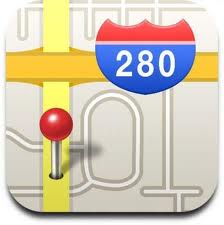
\includegraphics[scale=0.35]{plots/logo_apple_maps}
	
\includegraphics[scale=0.3]{plots/logo_facebook}
	
\includegraphics[scale=0.08]{plots/logo_yelp}
	
\includegraphics[scale=0.4]{plots/logo_mhealth}\\
	
\includegraphics[scale=0.5]{plots/logo_foursquare}
	
\includegraphics[scale=0.7]{plots/logo_google_now}
	
   \item \textbf{Phone sensing} fetches raw sensor data\ (e.g. from an accelerometer) and tries to extract high-level information from it\ (e.g. a user is walking).
   \item Such a process may have \textbf{high energy demands}, which is crucially important to mobile phone users.
   \item Energy-efficient phone sensing vs Tristan's results? or maybe HOW (what approach) ?!
  \end{itemize}
  

\includegraphics[scale=0.7]{plots/low_battery}

\includegraphics[scale=0.7]{plots/sad_face}

\mbox{}\framebreak
\section*{Solution}
\begin{itemize}
   \item different energy efficiency levels across devices [GRAPH the difference]
   \item however, accelerometer always better than others [GRAPH accelerometer]
   \item movement detection which leverages energy-efficient accelerometer to switch off GPS [MAYBE GRAPH]
   \item duty-cycling + adaptive towards the battery life
  \end{itemize}

\begin{figure}[H]
\includegraphics[scale=1]{plots/shared}
\caption{\label{p:shared} \footnotesize{Energy efficiency of shared sensors across different devices. The order of energy efficiency differs depending on a device e.g. Bluetooth is the most energy efficient sensor for HTC Desire and HTC Flyer, but not for Google Nexus 7.} }
\end{figure}

\begin{figure}[H]
\includegraphics[scale=1]{plots/acc_vs_loc}
\caption{\label{p:acc_vs_loc} \footnotesize{Energy efficiency levels of IEEE 802.11, GPS and accelerometer sensors across different devices. Acceleromter is more energy-efficient, but the difference is not substantial, and thus, efficient accelerometer sampling strategies needs to be introduced.} }
\end{figure}


\mbox{}\framebreak
\section*{Evaluation}
\begin{itemize}
   \item scenario I [GRAPH]
   \item scenario II [GRAPH]
  \end{itemize}
  
\begin{figure}[H]
\includegraphics[scale=1]{plots/locy_eval_inplace}
\caption{\label{p:locy_eval_place} \footnotesize{Energy efficiency levels of Locy library and Naive GPS Localization while a user is in place. Locy is more energy-efficient than baseline implementation for every phone.} }
\end{figure}


\begin{figure}[H]
\includegraphics[scale=1]{plots/locy_eval_other}
\caption{\label{p:locy_eval_other} \footnotesize{Energy efficiency levels of Locy library and Naive GPS Localization while a user is half of the time moving and the rest he is staying in one place. Locy is more energy-efficient than baseline implementation for every phone.} }
\end{figure}



\section*{Conclusions}
What does it mean?
[GIF HAPPY FACE + mobile phone + full battery]\\

\includegraphics[scale=0.7]{plots/full_battery}

\includegraphics[scale=0.7]{plots/happy_face}


\end{document}
